\section{Introduction}
\label{sec:intro}

Mental Disease\footnote{In this work, we will use `mental disorder' and `mental disease' interchangeably.} 
Detection (MDD) is of great practical value and social benefits, since mental disorders can greatly affect sufferers' life quality~\citep{Dreisbach2019systematic}.  
Lots of practices~\citep{coppersmith2015adhd,mowery2017understanding} indicate that social media posts, containing sufficient expressions about one's feelings and symptoms, can be an informative data source for text-based automatic MDD, which aims to predict whether a person suffers from certain mental diseases.

% \KZ{We are assuming MDD is a well-defined problem on social media posts? I think we need to either explain that will give a ref. What if a medical doctor reads this?} \MY{Agree with Kenny's comments, also you should restrain within text-based automatic MDD.}

However, traditional MDD methods \cite{yates2017depression, trotzek2018utilizing} process every post in the user's posting history, which can include many irrelevant or distracting posts. To avoid these noises, some prior works try to extract key posts by clustering \cite{zogan2021depressionnet} or semantic similarity \cite{zhang2022psychiatric}, but these heuristics can still introduce erroneous posts, affecting the subsequent MDD results. 

Moreover, comorbidity of several mental disorders is common \cite{ROCA2009Prevalence}. 
For instance, 75\% of depression patients in the surveyed population also suffer from anxiety disorder in their lifetime \cite{Femke2011Comorbidity}. 
Some research \cite{adam2013mental} further suggests that mental diseases lie along a spectrum, hence it is quite usual for one person to develop symptoms of several related mental disorders at the same time, and be diagnosed with multiple diseases. 
% \MY{Consider adding the reference once Zhiling mentioned that mental disorder is a spectrum so if you have one disorder, you are very much likely to have other related ones}
However, detecting multiple mental diseases simultaneously in the scenario of comorbidity is still under-explored. Most existing works focus on the detection of a single common disorder, such as depression \citep{losada2017erisk, lee2021micromodels}, ignoring the frequent comorbidity diagnosed in clinical practice.

To address these limitations, we aim to explore an approach to detect multiple mental disorders simultaneously in a comorbidity dataset, in which the diagnosed users can have one or more disorders. For simplicity, we refer to this detection task as \textbf{Multiple MDD} in this paper, and it can be viewed as a multi-label classification problem.
\begin{figure*}[t]
    \centering
    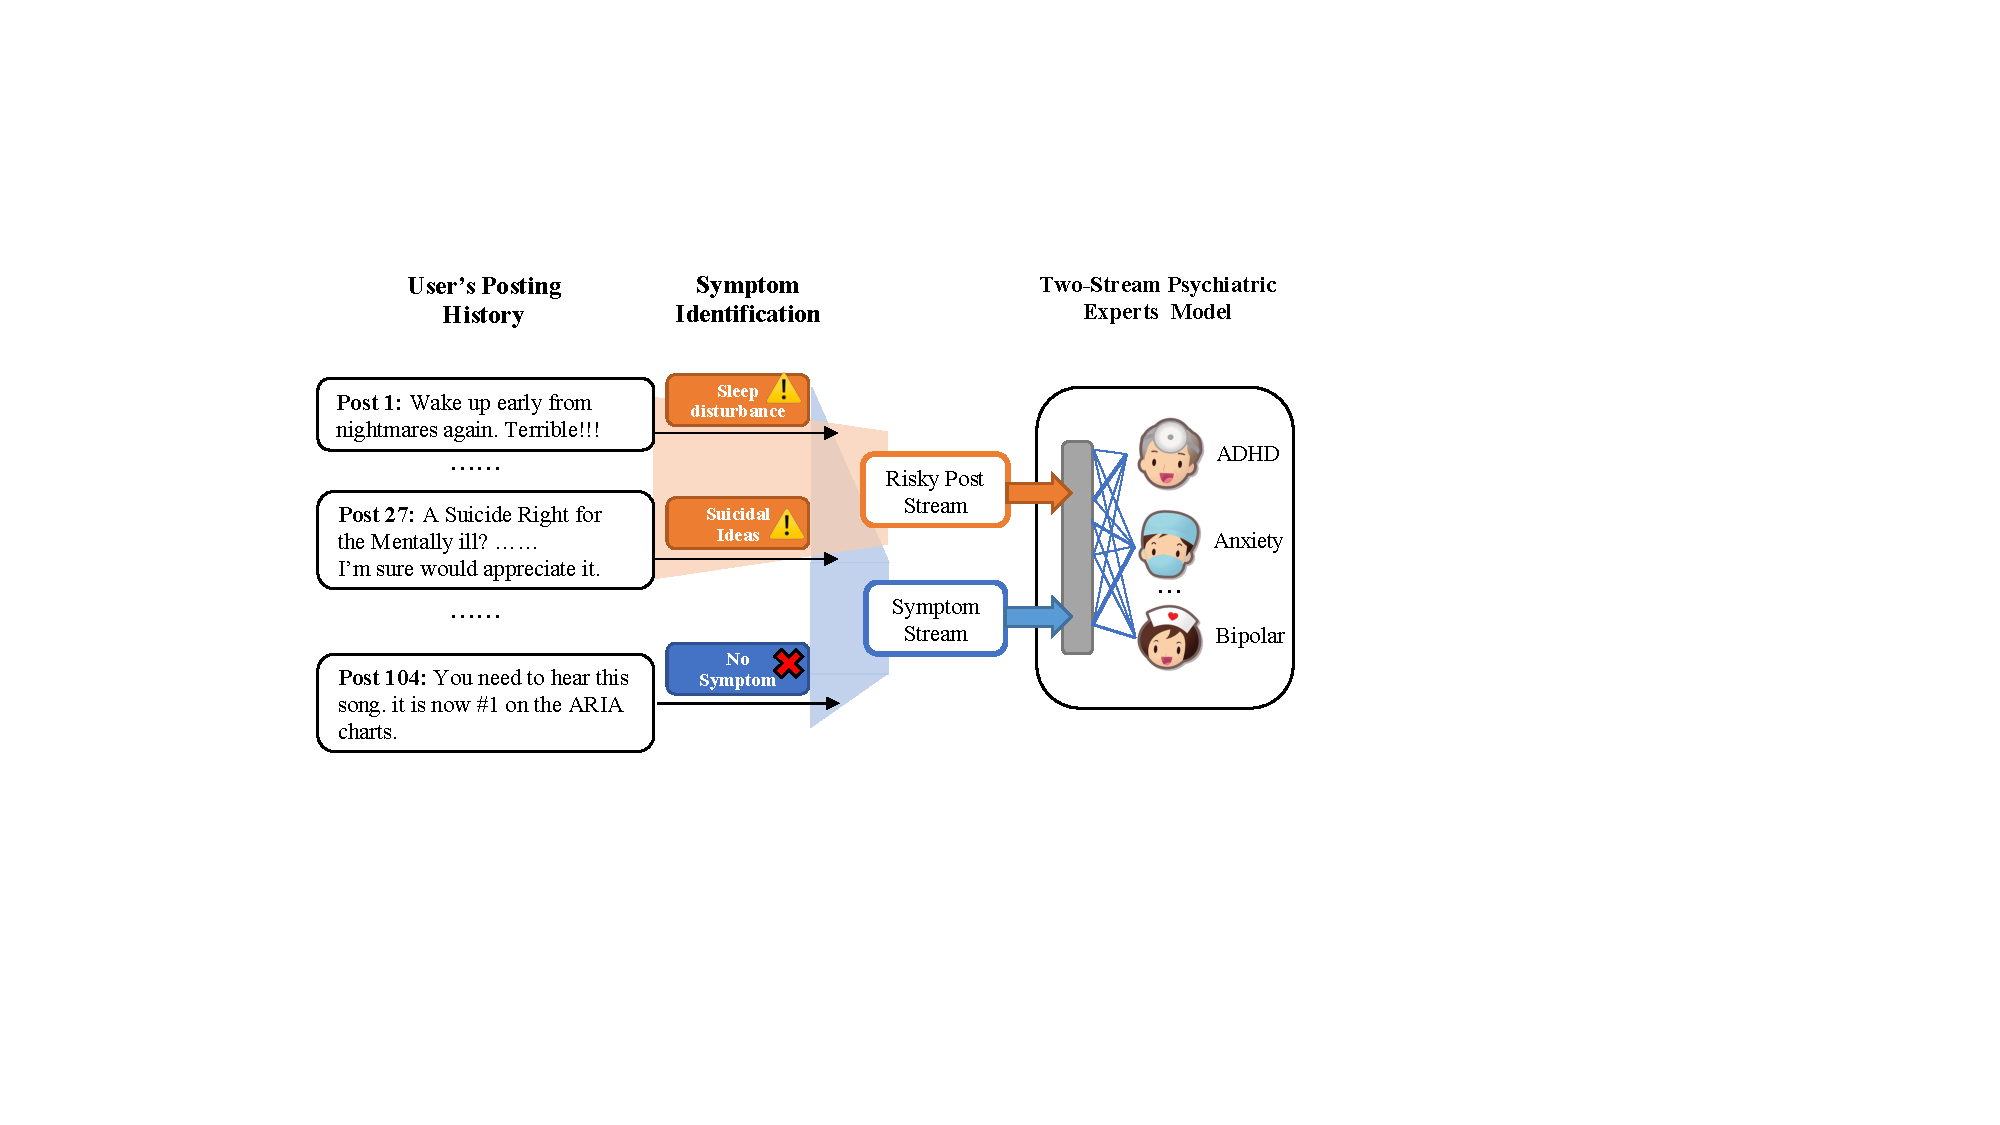
\includegraphics[width=1.7\columnwidth]{figures/pipeline.pdf}
    \caption{Psychiatric Experts Model with Symptom-based Risky Post Screening. Only posts highly related to psychiatric symptoms will be selected as diagnostic basis for further mental disease detection, which forms the risky post stream (the orange part). The symptom stream of a user contains all the symptom identification results from his/her whole posting history (the blue part), providing a more global view for the MDD model.}
    \label{fig:pipeline}
\end{figure*}

Intuitively, detecting multiple mental diseases can be challenging to resolve, as there are lots of overlapping clinical manifestations shared among different diseases, so the labels implicitly intersect with each other. Pioneering works on multiple MDD \cite{cohan2018smhd, sekulic2019adapting} commonly yield unsatisfying results as they simply use a shared model architecture for all diseases, which may not be strong enough to distinguish between diseases. \citet{Zhang2022SymptomIF} shows the effectiveness of implementing psychiatric symptom knowledge on multiple MDD, which is more interpretable and can outperform previous pure-text methods due to its better clinical grounding. However it detects each disease separately, ignoring the inner correlations between diseases, leading to unsatisfying results on rarer diseases like OCD.

In this work, we propose \textbf{PsyEx} (\textbf{Psy}chiatric \textbf{Ex}perts), a multi-task learning framework that can simultaneously detect 7 mental disorders\footnote{The 7 mental disorders are: ADHD, Anxiety Disorder, Bipolar Disorder, Depression, Eating Disorder, OCD and PTSD. Brief introductions about these disorders are included in Appendix \ref{apd:dis_intro}.} with a shared backbone and disease-specific structures to leverage the common characteristics of all diseases while still being able to capture their distinctions. This framework consists of two phases (see Figure \ref{fig:pipeline}). First, we utilize a symptom identification model that explicitly leverages psychiatric knowledge to obtain symptom features for the \textit{symptom stream}. The symptom features are also used to select posts that show high symptom risks. Then another \textit{risky post stream} implicitly learns clues for mental diseases from the semantics of the selected posts\footnote{We call them ``streams'' here because both symptom features and text features are arranged in chronological order.}. Therefore, these two streams can complement each other and improve interpretability based on domain knowledge. 
% We also utilize hierarchical structure to leverage the time clues of a user's posts in our proposed model.
% \KZ{We can call these two inputs two streams if the problem is an online detection problem, that is, the input keeps coming in. Another thing is that stream implies that it's a time series, so if the order of the posts does matter, then it's probably ok to call them streams.}
They are fed into the multiple MDD model which has 7 disease-specific psychiatric experts on top of a shared hierarchy network, so that the backbone can learn the shared knowledge between diseases, while each expert can focus on the characteristics of each specific disease. 
% \MY{Why is expert in quotation marks? Make it clear how the expert is realized, ``focus on their own domain'' still reads like a metaphor however you can explicitly say that each head attending to one specific disease}

% \MY{why text and symptom can complement each other? say it out that one is implicit and the other is explicit knowledge}
Experiments show that our method can achieve SOTA multiple MDD performance across 7 diseases and bring significant improvement to rarer diseases on which 
the baselines struggled heavily. 
Our main contributions are:
\begin{itemize}
    \item We successfully exploit psychiatric symptoms in 
this multiple MDD framework, including the symptom-based screening to facilitate a precise selection of risky posts, and the symptom stream to provide domain knowledge, together with a more holistic view of the entire posting history.  
    \item We propose a two-stream Psychiatric Experts Model for better multi-task learning of 7 mental disorders, which boosts the overall performance by better utilizing the distinctions and commonality among diseases. 
    \item With the interpretability enabled by symptom and disease-specific experts, we analyze the decision-making process of PsyEx, and further study the contribution of each symptom to the detection of different diseases. 
\end{itemize}







% myw starting like: Few works start to attend for multiple disease detection however commonly yield poor results due to the complexity of the problem and imbalanced data distribution.
%myw you don't have to say black-box nature - your method uses deep learning methods as well. start like: Interpretability is essential in clinical scenarios, however previous methods fail to ..., in particular on those false negative cases. For example, xxx
%myw different proportion is a weak argument, how about stressing on the entanglement of multiple diseases, e.g. stats in data suggesting #users have multiple diseases, and some are easily confused hence difficult to resolve in a single-disease detection model. This paragraph should state the real challenges and bottleneck of this work, and can relate to your method which is used to tackle these

% Thanks to the recent progress in mental disease symptom identification~\citep{Zhang2022SymptomIF}, we observed that \textit{symptom} can be a promising link between diseases, and provide more interpretability, since many psychiatrists also make a diagnosis based on the symptoms summarized in DSM-5 \cite{american2013diagnostic}. 
%myw this papragraph should better position as "shared knowledge and mixture of experts could help resolve previously-stated challenges", in two ways: disease-individual post selection and MoE modeling. This paragraph and be merged with the next one, stating the proposed method and its significance. 

% In this work, we proposed \textbf{PsyEx} (Psychiatric Experts), a new framework for MDD (Figure.\ref{fig:pipeline}), which simulates the diagnosis decision-making process of psychiatrists. 
% For the user's whole posting history, only posts highly-relevant to symptoms will be selected as \textit{risky posts}, providing interpretable basis for disease detection. 
% Then, we utilize multi-task learning of all diseases with multiple "experts" on top of a shared encoder, so that the backbone can learn the shared knowledge between diseases, while each expert can focus on their own domain. 
% Experiments show that our method can achieve SOTA MDD performance across 7 diseases and bring significant improvement to rarer classes where baselines struggled with. With the interpretability enabled by the multi-expert model and symptom-based risky posts, we can also study the contribution of each symptom to the detection of different diseases. 


